\textbf{P1)} \textcolor{red}{[Prueba 1 - 2024-20]} El sistema de dos bloques de masas $M_1$ y $M_2$, junto con una polea de masa $m$ y radio $r$, se libera desde el reposo, tal como indica la figura.
Asuma que las masas de los bloques satisfacen $M_2 > M_1$  para que se produzca movimiento, y que la inercia de la polea $ I_O = \frac{mr^2}{2}. $

\begin{enumerate}[a)]
	\item  Encuentre la relación entre la rapidez angular de la polea $\omega$ y la rapidez lineal de la cuerda $v$, asumiendo que no hay deslizamiento.
	\item  Asumiendo que el bloque $M_1$ ya ha perdido contacto con la mesa, realice los DCL relevantes, incluyendo todas las fuerzas externas sobre los cuerpos.
	\item  Calcule la aceleración angular $\alpha$ y las tensiones en la cuerda.
	\item  Encuentre la velocidad de los bloques justo antes de que $M_2$ golpee la mesa.
\end{enumerate}

\center{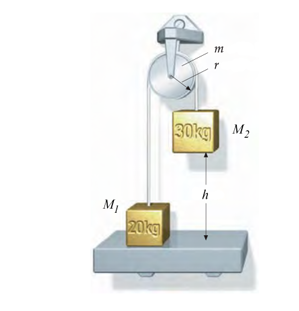
\includegraphics[width=0.5\textwidth]{imagenes/pregunta 1 ayudantia 5.PNG}}

\newpage

\textbf{P2)} Un objeto cil\'indrico de masa $M$, radio exterior $R$ y con una perforaci\'on cil\'indrica conc\'entrica de radio $r$, descansa sobre una superficie horizontal rugosa. De su orificio central (que no presenta fricci\'on) se sujeta una cuerda inextensible y de masa despreciable. Esta cuerda pasa por una polea fija y luego por una polea m\'ovil que sostiene un bloque de masa $m$, tal como se muestra en la figura. El sistema se libera desde el reposo.

\begin{enumerate}[a)]
	\item Suponga que el cilindro rueda sin resbalar. Establezca la relaci\'on geom\'etrica entre la aceleraci\'on lineal $a_c$ del centro de masa del cilindro y la aceleraci\'on lineal $a_b$ del bloque. Asimismo, escriba la relaci\'on entre la aceleraci\'on angular $\alpha$ del cilindro y $a_c$.
	\item Determine una expresi\'on algebraica para la aceleraci\'on lineal $a_b$ del bloque, expresando su resultado en t\'erminos de $M$, $m$, $R$, $r$ y $g$.
	\item Considere que el cilindro perforado tiene una masa $M = 16,0\,\mathrm{kg}$, un radio exterior $R = 40,0\,\mathrm{cm}$ y un radio interior $r = 20,0\,\mathrm{cm}$. Si el coeficiente de roce est\'atico entre el cilindro y la mesa es $\mu_E = 0{,}250$, determine el valor m\'aximo de la masa del bloque $m_{b,\max}$ que se puede colgar del sistema para garantizar que el cilindro ruede sin resbalar.
	\item Ahora suponga ahora que, por nuevos requerimientos operacionales, es estrictamente necesario utilizar un bloque de masa $m = 50{,}0\,\mathrm{kg}$. Manteniendo las caracter\'isticas del cilindro intactas, determine el coeficiente de roce est\'atico m\'inimo $\mu_{E,\min}$ que debe proporcionar el recubrimiento de la mesa para garantizar que el cilindro ruede sin resbalar bajo esta exigente carga.
\end{enumerate}

\center{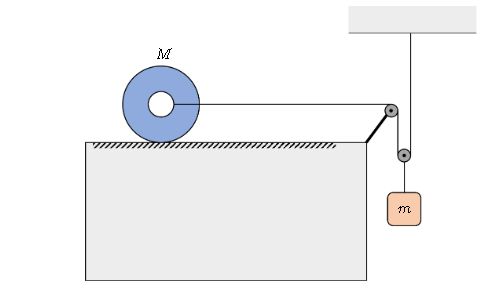
\includegraphics[width=0.75\textwidth]{imagenes/a5p2.PNG}}